\documentclass[11pt]{report}
\usepackage{amsmath, bm, xcolor, graphicx, listings}
\usepackage{courier} %for listings
\usepackage{caption}
\usepackage{subcaption}
\lstset{basicstyle=\footnotesize\ttfamily,breaklines=true} %listing font settings
%\lstset{framextopmargin=50pt} %listing font settings
\usepackage[english]{babel}
\setlength\parindent{0pt} %remove indentation in new paragraphs


\begin{document}
\title{\textbf{CParticle}}
\author{Nikos Tryfonidis}
\date{2015}

\maketitle

\begin{abstract}
The current report summarizes the structure, use and results of \emph{CParticle}, a charged particle simulation code written in C. \emph{CParticle} simulates the motion of a charged particle (ion or electron) in electromagnetic fields, that are specified by the user in vector form (Cartesian coordinates). First, a small introduction to the code will be given in chapter 1. Afterwards, the structure of the code will be reviewed in chapter 2. Finally, a number of test cases will be shown, as examples on how to use the code while also verifying its correctness.
\end{abstract}

\tableofcontents

\chapter{Introduction}
CParticle is a three-dimensional charged particle simulation code written in C. The code was written as part of my PhD project, in order to gain insight into the numerical simulation of charged particle motion and eventually to be integrated into a Particle-In-Cell code, as the particle "pusher".
\newline

In this chapter, a brief introduction to the code will be made, with instructions on how to compile, run and view the simulation results.

\section{Compiling and Running}
The code should compile without problems on any machine able to compile C code with "make". To compile, simply go to the main directory, where the makefile is located, and type "make". This will build the executable (named "\emph{cparticle}") in the same directory. To run the code, simply run the executable from the command line, providing four (4) arguments:

\begin{lstlisting}
./cparticle <particle type> <total time> <dt> <output interval>
\end{lstlisting}

\begin{description}
\item[particle type] Choose \emph{"i"} for ion (positive charge) or \emph{"e"} for electron (negative charge).
\item[total time] The total time units for the particle motion to be simulated. 
\item[dt] The timestep for the numerical solver.
\item[output interval] Number of steps between output.
\end{description}

For example, if we want to simulate the motion of an electron for $100$ time units, with a timestep of $0.001$, and want output every 10 timesteps, we will run as:

\begin{lstlisting}
./cparticle e 100 0.001 10
\end{lstlisting}

Output is written in the "output" directory, in two ".txt" files:

\begin{description}
\item[output.txt] Contains output in seven columns. The first column is the time for every output step of the simulation. The next 3 columns are the position of the particle ($x, y, z$). The final 3 columns are the velocity of the particle ($v_x, v_y, v_z$).
\item[energy.txt] The kinetic energy of the particle for every output step.
\end{description}

\section{Visualization}
Visualization of the results is handled with Python scripts that use NumPy and matplotlib, two well-known packages for scientific computing in Python.

These can be easily installed in any Linux system, for example in Ubuntu:

\begin{lstlisting}
sudo apt-get install python-numpy python-matplotlib
\end{lstlisting}

The following visualization scripts can be found in the "plot" directory:

\begin{description}
\item[plot\_xyz.py] Creates the plot of a single chosen coordinate (position, velocity) versus time, and also a 3D plot trajectory of the particle. 
\item[animate.py] Creates a 3D animation of the particle trajectory.
\item[plot.py] This script is called by \emph{plot\_xyz.py}. The user does not have to edit or use this directly.
\end{description}

After running the program, to create the plots, the user can simply go to the \emph{plot} directory and do the following:

\begin{lstlisting}
python plot_xyz.py
\end{lstlisting}

This will produce the $x(t)-t$ and $v_x(t)-t$ plots in one figure, and also the phase-space plot $v_x(t) - x(t)$ in another. After the user closes these two figures, the 3D trajectory plot of the particle motion will be created.

To create the animation of the motion, the user can run the \emph{animate.py} script:

\begin{lstlisting}
python animate.py
\end{lstlisting}

This will show the animated motion of the particle. If the user wants to save the animation, he should uncomment the last lines in the script (the lines after the comment saying "save animation"), while also commenting out the \emph{"plt.show()"} line. Please note that in order to save the animation, the script uses \emph{ffmpeg}. This has to be installed and be reachable in \emph{/usr/bin/}.
 
\chapter{Code Structure}
In this chapter, the structure of the code will be briefly reviewed. First, a description of the source files and code will be given, followed by a description of the data structures used. Afterwards, an outline of how to create a simulation (setting up the electromagnetic fields etc).

\section{Directories}
The project consists of the following directories:

\begin{description}
\item[src] Contains the source files of the project. These will be described in more detail in the next section.
\item[headers] Contains headers needed for the source files. Every source files has its corresponding header file, with function headers for the functions that are callable \emph{outside} their source file.
\item[output] Output files are written here by the program.
\item[documentation] Contains the current documentation.
\item[plot] Contains the Python plotting scripts.
\item[obj] Contains object files (.o).
\end{description}

Also, the \emph{"input.txt"} file, in the main directory of the project, contains initial conditions for the particle (3 position coordinates and 3 velocity coordinates).

\section{The Code}
The code is contained in the \emph{src} directory, in the following source files:

\begin{description}
\item[main.c] The main source file. Reads input, allocates memory, calls the solver wrapper and finally writes the output.
\item[fields.c] The electromagnetic field functions. Contains the Electromagnetic Force function calculator (\emph{FLorentz}), a cross product evaluating function (\emph{cross}), and functions for the user to set the Electric and Magnetic fields (\emph{EField and BField}, respectively).
\item[motion.c] The solver wrapper function (\emph{motion}) in this file calls the solver for the required number of steps and writes output in memory for every interval requested.
\item[solver.c] Contains the numerical solver function \emph{RK4\_ motion3D}. This function calculates the particle motion for one timestep and returns the particle with updated coordinates. The numerical method used is the \emph{4th order Runge Kutta} method.
\item[memory.c] Contains the \emph{array2D\_ contiguous} function, that dynamically allocates a 2D array contiguously in memory and \emph{free\_ array2D\_ contiguous}, which frees memory allocated in the previous way.
\item[io.c] Contains functions that read input from the input file and the command line, print the problem parameters to the screen and write output to memory and output files.
\end{description}

The following header files in \emph{headers/struct.h} are also of interest:
\begin{description}
\item[definitions.h] Contains values for particle (ion or electron) charge and mass. These are currently set to 1.0 or -1.0 respectively.
\item[struct.h] Contains the structure definitions for the program. These are described in the next section.
\end{description}
\newpage
\section{Data Structures}
The program uses the following data structures, defined in \emph{headers/struct.h}:

\begin{description}
\item[vector3D] A 3D vector, consisting of 3 double variables, one for each coordinate. A very useful data structure for this program, vector structures are used in the \emph{particle} structure and by the \emph{field} functions in \emph{field.c}.
\begin{lstlisting}
struct vector3D {
    double x;
    double y;
    double z;
};
\end{lstlisting}
\item[particle] The main data structure of the program. Contains information about the particle whose motion is simulated. \emph{Position} and \emph{velocity} are \emph{vector structures}. Also contains the particle \emph{charge} and \emph{mass}. These could have been defined as macros, but as the program aims to be part of a Particle-In-Cell code simulating many particles (both ions and electrons), this information was included in the particle structure.
\begin{lstlisting}
struct particle {
    struct vector3D r;
    struct vector3D v;
    double q;
    double m;
};
\end{lstlisting}

\item[time] A structure containing the time parameters of the program, in order to pass them in a neat way 
to functions.
\begin{lstlisting}
struct time {
  double totalTime;
  double dt;
  int output_interval;
  int totalTimeSteps;
  int nOutput;
};
\end{lstlisting}
\end{description}
\newpage
\section{The Numerical Method}
The program essentially solves the charged particle equations of motion, following Newton's 2nd Law formalism:
\begin{equation}
\frac{d^2 \overrightarrow{r}}{dt^2} = \frac{\overrightarrow{F_L}}{m}
\end{equation}

where
\begin{equation}
\overrightarrow{F_L} = q\left(\overrightarrow{E} + \overrightarrow{v} \times \overrightarrow{B} \right).
\end{equation}

Runge-Kutta (4th order) was chosen as the numerical method for the motion for the particle. Being a multistage method, Runge-Kutta requires the calculation of the right-hand-side of (2.1) for each of the four stages it calculates. A decision was made to write the solver function in the clearest possible way, avoiding switches and other methods that would make it more compact but much less clear.
\newline

A detailed analysis of Runge-Kutta is outside the scope of this report, but can be found in most Numerical Analysis textbooks dealing with the numerical solution of Ordinary Differential Equations, such as \cite{leveque}.

\newpage
\section{Setting Up a Simulation}
To set up a particular problem, the user has to do the following actions:

\begin{itemize}
\item Set the desired Electric and Magnetic fields in \emph{fields.c}.
\item Set the definitions for particle mass and charge in in \emph{headers/definitions.h}.
\item Compile the program by typing "make".
\item Set the desired initial conditions for the particle in \emph{"input.txt"}.
\item Run the program, as described in the introduction, specifying the time parameters.
\end{itemize}

After running the program, output is written in the \emph{output} directory and can be visualized with the Python scripts in the \emph{plot} directory, as shown in the introduction.

\chapter{Examples}
In this chapter, a number of representative problems will be shown. A detailed analysis and study of charged particle motion is outside the scope of this report, but excellent references include \cite{goldston}, \cite{freidberg} and \cite{bellan}. Detailed analysis of every example shown in the following sections can be found in the previous references.

\section{Gyromotion}
In this section we will show the simulation results of the motion of a charged particle in a uniform magnetic field $B$, with no electric field. This motion is known as \emph{gyromotion} or \emph{cyclotron motion}, because the particle performs a circular motion around the magnetic field lines. 
\newline

One fundamental quantity of the gyromotion is the \emph{cyclotron frequency} (also known as \emph{Larmor frequency} or \emph{gyro-frequency}), which is the angular frequency of the circular motion of the particle:

\begin{equation}
\omega_c = \frac{|q|B}{m}
\end{equation}

where $q$ is the particle charge, $B$ is the magnitude of the magnetic field and $m$ the mass of the particle.
\newline

Another important quantity of the cyclotron motion is the \emph{cyclotron radius} (or \emph{gyroradius} or \emph{Larmor radius}), the radius of the circular motion of the charge:

\begin{equation}
r_c = \frac{m u_{\bot}}{|q|B}
\end{equation}

where $u_{\bot}$ is the magnitude of the particle's velocity \emph{perpendicular} to the magnetic field.
\newline

As a general rule, we expect charged particles to perform a circular motion around the magnetic field lines, with frequency as in (3.1) and radius as in (3.2). In addition, if we point our two thumbs along the direction of the magnetic field, ions rotate in the direction of our left-hand fingers, while electrons rotate in the direction of our right-hand fingers. 

\subsection{Ion Gyromotion}
We will now simulate the gyromotion of an ion in a uniform magnetic field. For simplicity, we will assume that $\bm{B} = B_0 \hat{\bm{z}}$ and that $B_0 = 1$. To do this, we go to \emph{src/fields.c} and edit the \emph{BField} function in this way:

\begin{lstlisting}
struct vector3D BField (struct vector3D r, double t)
{
  struct vector3D B;

  B.x = 0.0;
  B.y = 0.0;
  B.z = 1.0;

  return B;
}
\end{lstlisting}

We also set all components of the electric field to zero (\emph{EField} function in the same source file). Finally, the ion mass and charge are set equal to $1.0$ (this can be done in \emph{headers/definitions.h}).
\newline 

We compile the program by typing \emph{"make"} in the main project directory. After our executable is ready, we can enter our desired initial conditions in \emph{input.txt}. If we want the particle's starting position to be at $r_0 = (0,0,0)$ and its initial velocity to be $v_0 = (1, 1, 1)$, we edit the input file as follows:

\begin{lstlisting}
r 0.0 0.0 0.0
v 1.0 1.0 1.0
\end{lstlisting}

From the parameters given above, we expect a gyrofrequency 
\begin{equation}
\omega_c = \frac{|q|B}{m} = \frac{1 \cdot 1}{1} = 1
\end{equation}

and thus a period of the circular motion

\begin{equation}
T_c = \frac{2 \pi}{\omega_c} = \frac{2 \pi}{1} = 2 \pi
\end{equation}

and a gyroradius of 
\begin{equation}
r_c = \frac{m u_{\bot}}{|q|B} = \frac{1 \cdot \sqrt{u_x^2 + u_y^2}}{|1| \cdot 1}
= \sqrt{1^2 + 1^2} = \sqrt{2} \simeq 1.414
\end{equation}

We expect a helical motion and, since we are simulating an ion (positive charge), a clockwise circular motion if we view space from the z-axis top-down.
\newline

We run the program as follows (aiming for 10 periods):

\begin{lstlisting}
./cparticle i 62.8 0.001 10
\end{lstlisting}

Once the simulation is finished, output is written in the \emph{output} directory. We can now produce some plots to visualize the output, using the Python visualization scripts in the \emph{plot} directory.
\newline

First, by running the script \emph{plot\_xyz.py} we can produce $x(t) - t$ and $v_x(t) - t$ plots. We can choose the desired components to plot, as indicated inside the script. For example, if we want to plot the $x$ component of the motion, we edit the \emph{plot\_ xyz.py} script as follows:

\begin{lstlisting}
plot1D(t, x, v_x)
\end{lstlisting}

We run the script as follows:

\begin{lstlisting}
python plot_xyz.py
\end{lstlisting}

Below we show the collected output of the program, for all components ($x, v_x$ etc) separately. Afterwards, we show the 3D plot of the trajectory. Finally, we will show the figure of the completed animation, which can be created by running the \emph{animate.py} script as follows:

\begin{lstlisting}
python animate.py
\end{lstlisting}

\begin{figure}[!ht]
  \centering
    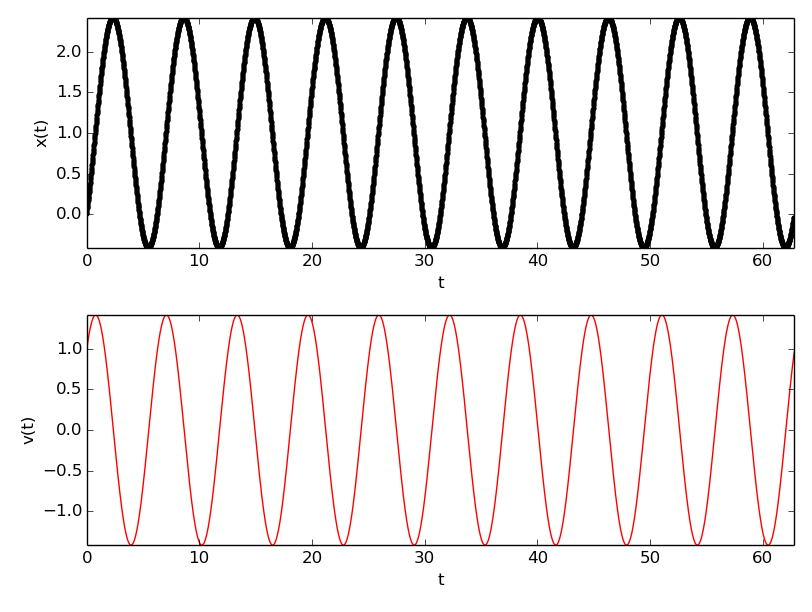
\includegraphics[width=0.75\textwidth]{images/gyro_ion_x}
    \caption{$x(t)$, $v_x(t)$ plot. We see the expected sinusoidal motion of the ion along $x$. Notice that the ion completes the expected number of cyclotron periods (10) and the ion's gyroradius is the expected $r_c \simeq 1.414$.}
\end{figure}

\begin{figure}[!ht]
  \centering
    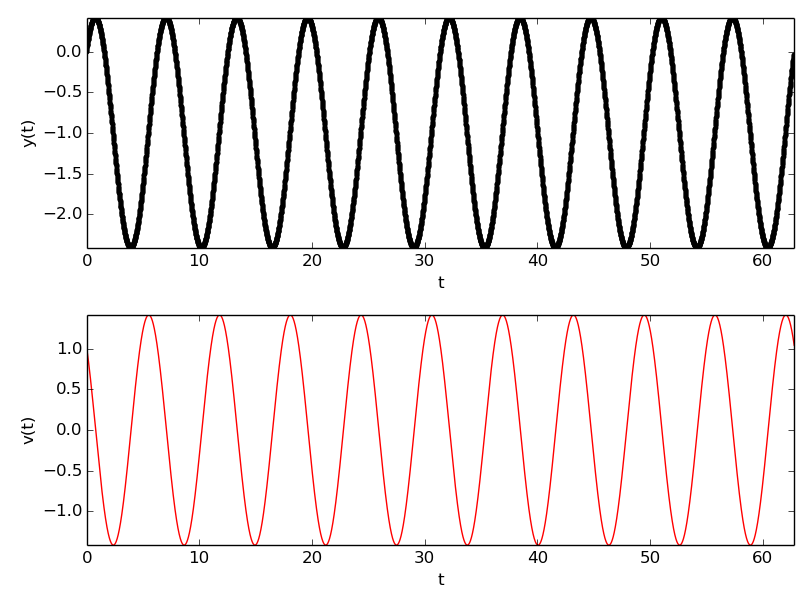
\includegraphics[width=0.75\textwidth]{images/gyro_ion_y}
     \caption{$y(t)$, $v_y(t)$ plot. We see again the expected sinusoidal motion of the ion along $y$. The same number of cyclotron periods (10) is completed and the ion's gyroradius is the expected $r_c \simeq 1.414$.}
\end{figure}

\begin{figure}[!ht]
  \centering
    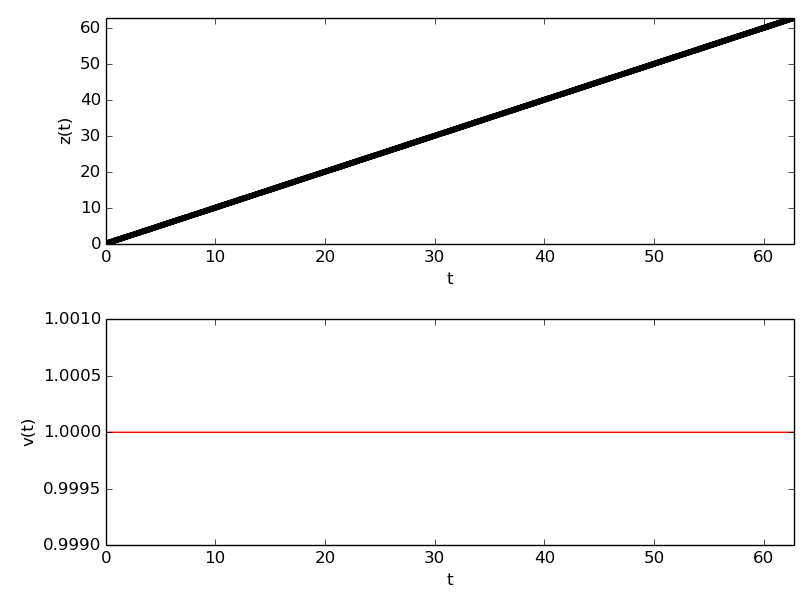
\includegraphics[width=0.75\textwidth]{images/gyro_ion_z}
     \caption{$z(t)$, $v_z(t)$ plot. The ion's motion along  is unaffected by the magnetic field, as expected. The ion moves along $z$ with its initial, constant velocity.}
\end{figure}

\begin{figure}[!ht]
  \centering
    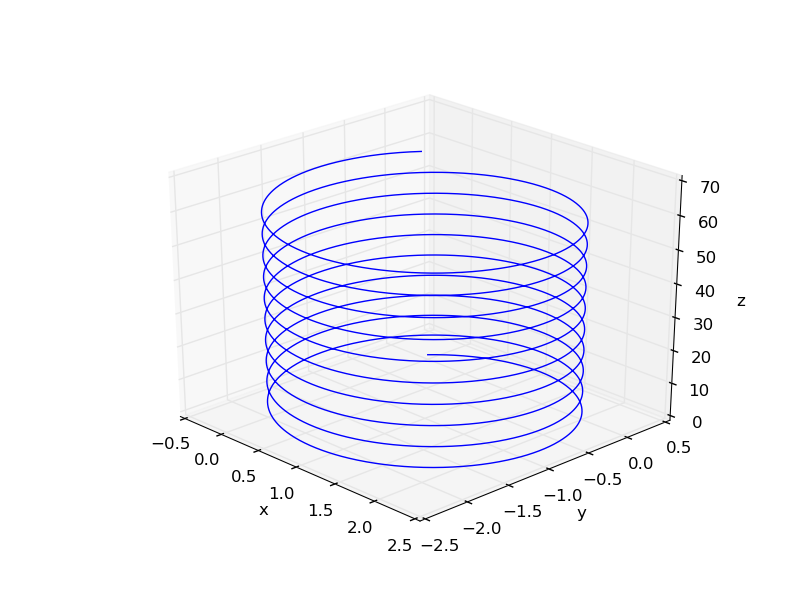
\includegraphics[width=0.75\textwidth]{images/gyro_ion_3d}
     \caption{The 3D plot of the ion's trajectory. We see the expected helical motion for $\bm{B} = B_0\hat{\bm{z}}$, \emph{clockwise} (left-hand rule), as expected}
\end{figure}

\begin{figure}[!ht]
  \centering
    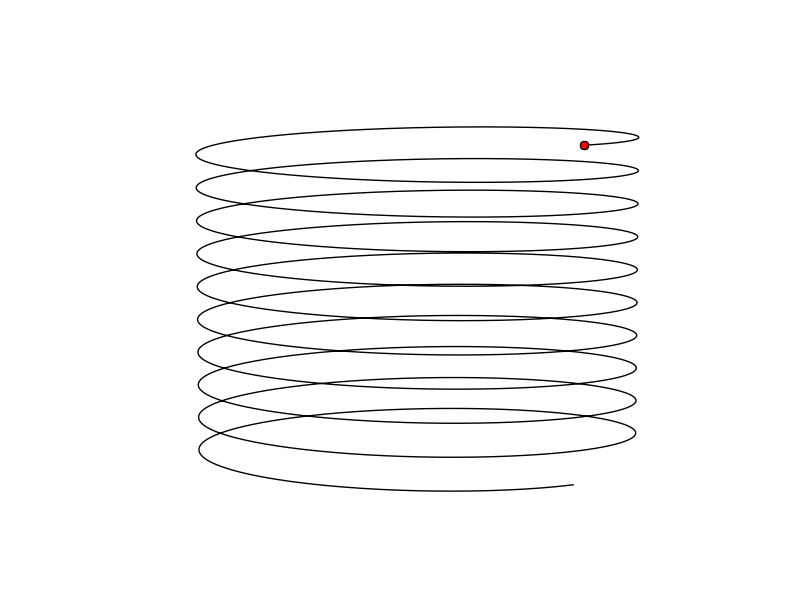
\includegraphics[width=0.75\textwidth]{images/gyro_ion_3d_anim}
     \caption{The completed animation of the ion's trajectory. The user can create the animation by running the \emph{animate.py} script.}
\end{figure}

\newpage

\subsection{Electron Gyromotion}
In this subsection we will show how to set up and run an electron's gyromotion, and the visualization results. The simulation and quantities are similar to the previous section (we are keeping $q_e = 1.0$ and $m_e = 1.0$ for simplicity). The only difference is that for an electron's gyromotion, we expect to see an anti-clockwise circular motion, viewing space from the z-axis top-down. 
\newline

We do not actually need to recompile the program. Keeping the same initial conditions in \emph{input.txt}, we run the program, simply changing $i$ to $e$, as follows:

\begin{lstlisting}
./cparticle e 62.8 0.001 10
\end{lstlisting}

We will only show the 3D trajectory plot here, due to the similarity with the ion motion shown previously.

\begin{figure}[!ht]
  \centering
    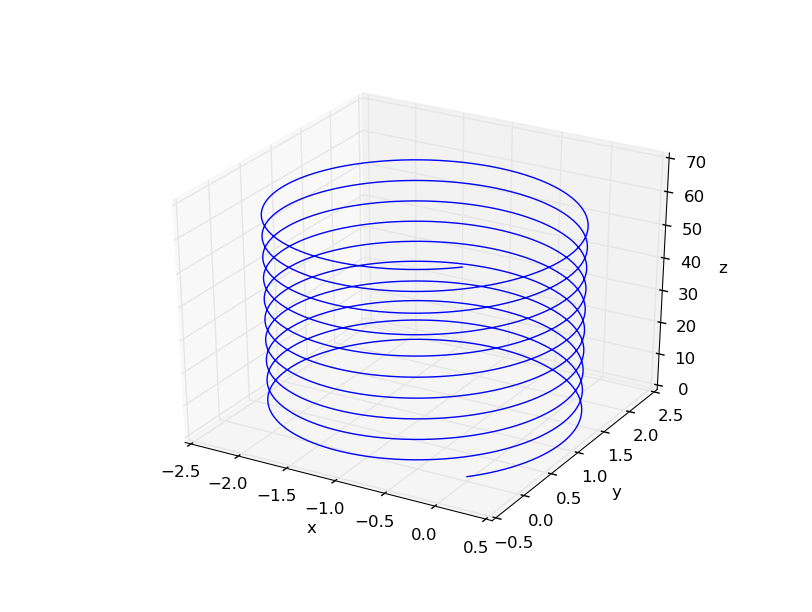
\includegraphics[width=0.75\textwidth]{images/gyro_electron_3d}
     \caption{The 3D plot of the electron's trajectory. We see the expected helical motion for $\bm{B} = B_0\hat{\bm{z}}$, \emph{anti-clockwise} (right-hand rule), as expected.}
\end{figure}

\newpage
\section{$\bm{E} \times \bm{B}$ Drift}
When a charged particle moves in uniform $\bm{E}$ and $\bm{B}$ fields, along with the gyromotion we previously saw, it exhibits what is commonly known as a \emph{drift} velocity:

\begin{equation}
\bm{v}_D = \frac{\bm{E} \times \bm{B}}{B^2}
\end{equation}

In other words, this motion is identical to the gyromotion that we encountered in the previous section, plus a constant velocity $\bm{v}_D$ as shown in (3.6). In this section we will simulate this drift motion for an ion and an electron. What is interesting is the fact that ions and electrons drift in the same direction in $\bm{E}, \bm{B}$ fields. A detailed analysis $\bm{E} \times \bm{B}$ drift motion can be found in most plasma physics books; however, the analysis of \cite{freidberg} is, in my opinion, one of the clearest.

\subsection{Ion Drift Motion}
We will set the electric field along the $y$ axis and the magnetic field along the $z$ axis, for simplicity:

\begin{align}
\bm{E} & = E_0 \hat{\bm{y}} \\
\bm{B} & = B_0 \hat{\bm{z}}\\
E_0 = 0.1, & \quad \quad B_0 = 1.0
\end{align}

In this way, we expect the following drift velocity:

\begin{equation}
\bm{v}_D = \frac{\bm{E} \times \bm{B}}{B^2} = 0.01 \hat{\bm{x}}
\end{equation}

We set the desired electric and magnetic fields (3.7) - (3.9), in \emph{src/fields.c}:

\begin{lstlisting}
struct vector3D EField (struct vector3D r, double t)
{
  struct vector3D E;

  E.x = 0;
  E.y = 0.1;
  E.z = 0;

  return E;
}

struct vector3D BField (struct vector3D r, double t)
{
  struct vector3D B;

  B.x = 0.0;
  B.y = 0.0;
  B.z = 1.0;

  return B;
}
\end{lstlisting}

We compile and, using the same initial conditions as in the previous section, we run the program:

\begin{lstlisting}
./cparticle i 62.8 0.001 10
\end{lstlisting}

Below we can see the visualization results of the program:

\begin{figure}[!ht]
  \centering
    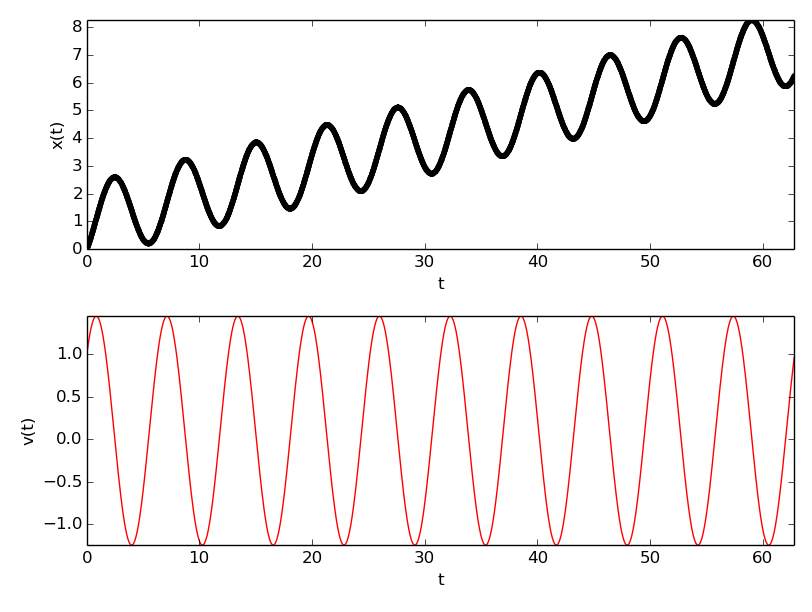
\includegraphics[width=0.75\textwidth]{images/drift_ion_x}
    \caption{$x(t)$, $v_x(t)$ plot. We see the sinusoidal motion of the ion along $x$, plus the expected drift velocity. Notice that the ion completes the expected number of cyclotron periods (10).}
\end{figure}

\begin{figure}[!ht]
  \centering
    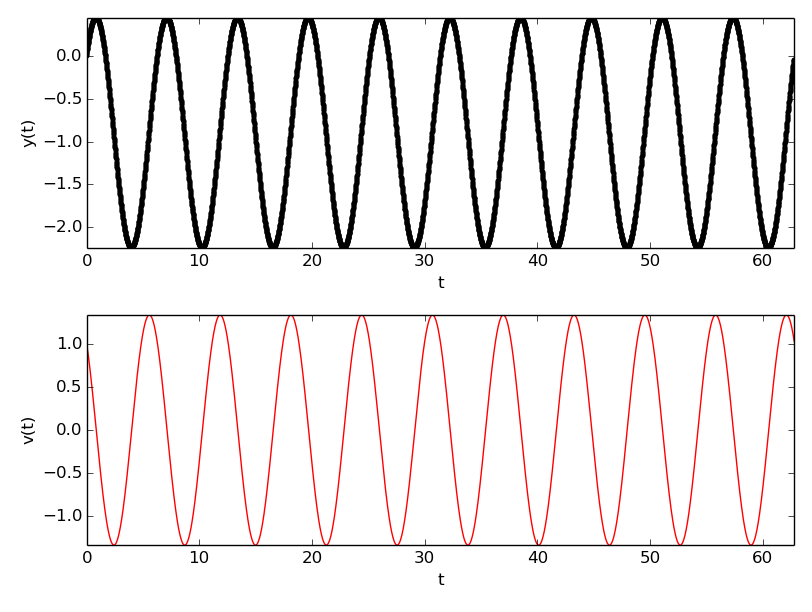
\includegraphics[width=0.75\textwidth]{images/drift_ion_y}
     \caption{$y(t)$, $v_y(t)$ plot. We see again the expected sinusoidal motion of the ion along $y$, without any drift motion along $y$, as expected. The same number of cyclotron periods (10) is completed.}
\end{figure}

\begin{figure}[!ht]
  \centering
    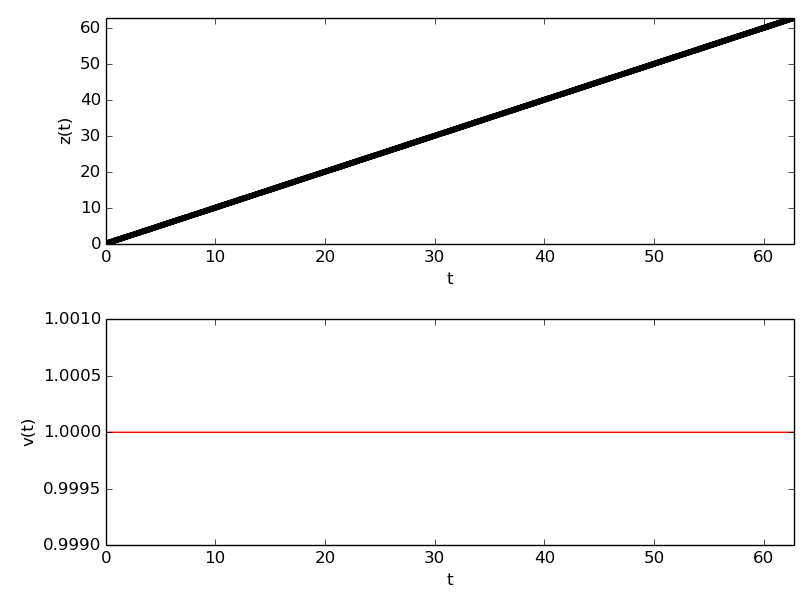
\includegraphics[width=0.75\textwidth]{images/drift_ion_z}
     \caption{$z(t)$, $v_z(t)$ plot. The ion's motion along  is unaffected by the magnetic field, as expected. The ion moves along $z$ with its initial, constant velocity.}
\end{figure}

\begin{figure}[!ht]
  \centering
    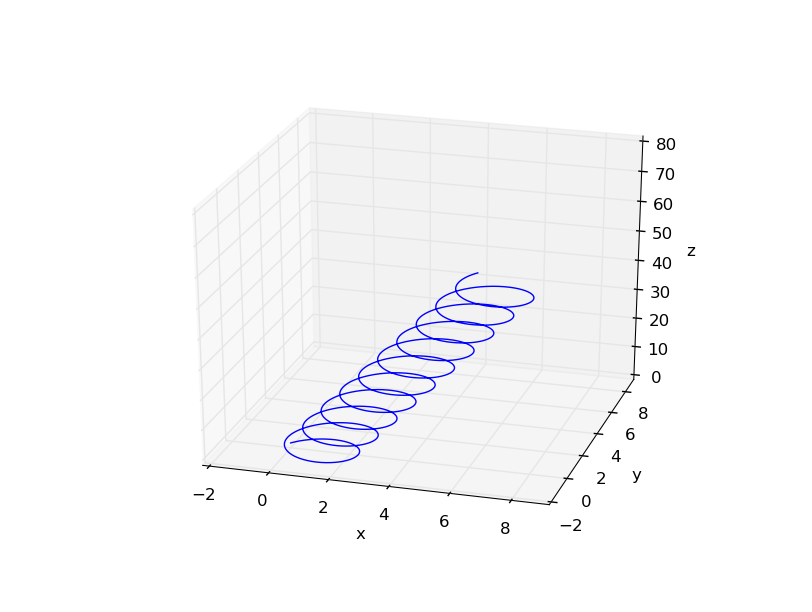
\includegraphics[width=0.75\textwidth]{images/drift_ion_3d}
     \caption{The 3D plot of the ion's trajectory. We see the expected helical motion for $\bm{B} = B_0 \hat{\bm{z}}$, drifting along the $\hat{\bm{x}}$ axis.}
\end{figure}

\newpage

\subsection{Electron Drift Motion}
In this section we will show the simulation of an electron's drift motion. We will keep everything similar to the previous section and we will simply run for an electron, as follows:

\begin{lstlisting}
./cparticle e 62.8 0.001 10
\end{lstlisting}

Below we can see the 3D trajectory of the electron (other plots are similar to those of the previous section).

\begin{figure}[!ht]
  \centering
    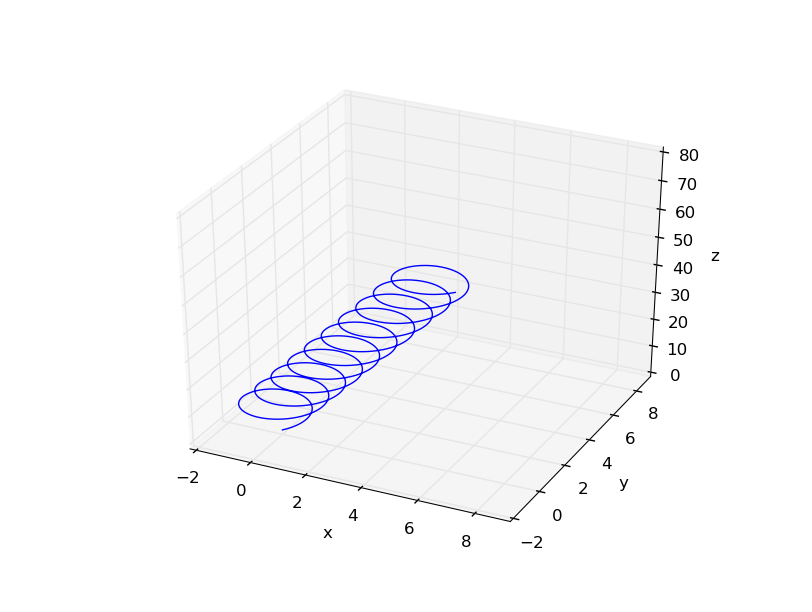
\includegraphics[width=0.75\textwidth]{images/drift_electron_3d}
     \caption{The 3D plot of the electron's trajectory. We see the expected helical motion for $\bm{B} = B_0 \hat{\bm{z}}$, drifting along the $\hat{\bm{x}}$ axis, with the same drift velocity as the ion in the previous section.}
\end{figure}

\section{$\nabla \bm{B}$ Drift}
When moving inside a non-uniform magnetic field with a gradient $\nabla B$, a charged particle also exhibits a drift, commonly known as a \emph{gradient drift}:

\begin{equation}
\bm{v}_{grad} = \pm \frac{u_{\bot}^2}{2\omega _c} \frac{\bm{B} \times \nabla B}{B^2}
\end{equation}

where the sign corresponds to the sign of the particle's charge; contrary to $\bm{E} \times \bm{B}$ drifts, in $grad-B$ drifts ions and electrons drift in opposite directions.
\newline

In this section, we will simulate the drift motion of an ion and an electron. We set up the Electric and Magnetic fields in \emph{fields.c} as follows: 

\begin{lstlisting}
struct vector3D EField (struct vector3D r, double t)
{
  struct vector3D E;

  E.x = 0;
  E.y = 0;
  E.z = 0;

  return E;
}

struct vector3D BField (struct vector3D r, double t)
{
  struct vector3D B;

  B.x = 0.0;
  B.y = 0.0;
  B.z = r.y;

  return B;
}
\end{lstlisting}

and we start the particle from position $\bm{r}_0 = (0, 1, 0)$ and with initial velocity $\bm{v}_0 = (0.1, 0.1, 0.1)$, editing the input file \emph{input.txt} as follows:

\begin{lstlisting}
r 0.0 1.0 0.0
v 0.1 0.1 0.1
\end{lstlisting}

These initial conditions ensure that the motion is kept simple enough for the illustration purposes of this report. With the above, we expect the following drift directions for ions and electrons, respectively:

\begin{align*}
Ions:& \quad \quad \bm{v}_D \sim -\bm{\hat{x}}\\
Electrons:&  \quad \quad \bm{v}_D \sim +\bm{\hat{x}}
\end{align*}
\newpage

\subsection{Ion Grad-B Drift}
We run the program as follows:

\begin{lstlisting}
./cparticle i 62.8 0.001 10
\end{lstlisting}

Below we can see the visualization results of the ion grad-B drift:

\begin{figure}[!ht]
  \centering
    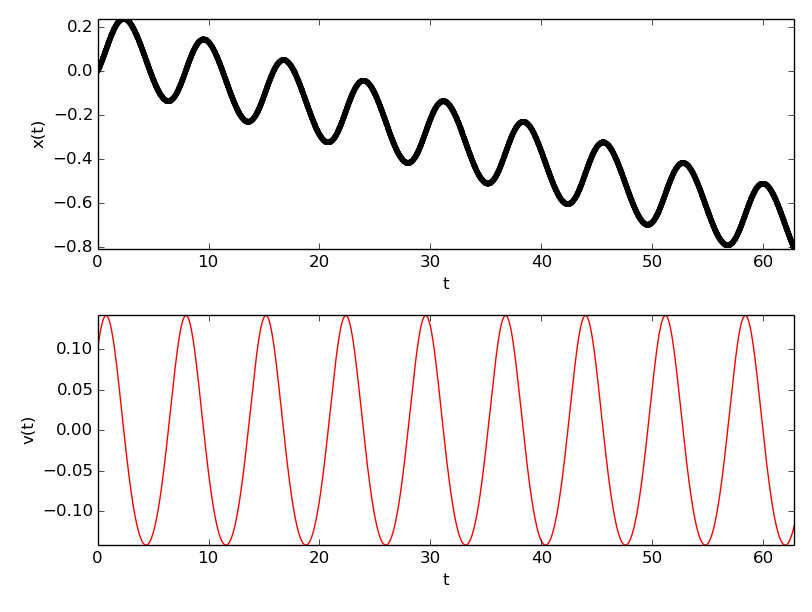
\includegraphics[width=0.75\textwidth]{images/gradB_ion_x}
    \caption{$x(t)$, $v_x(t)$ plot. We see the sinusoidal motion of the ion along $x$, plus the expected drift velocity towards the negative $x$ axis.}
\end{figure}

\begin{figure}[!ht]
  \centering
    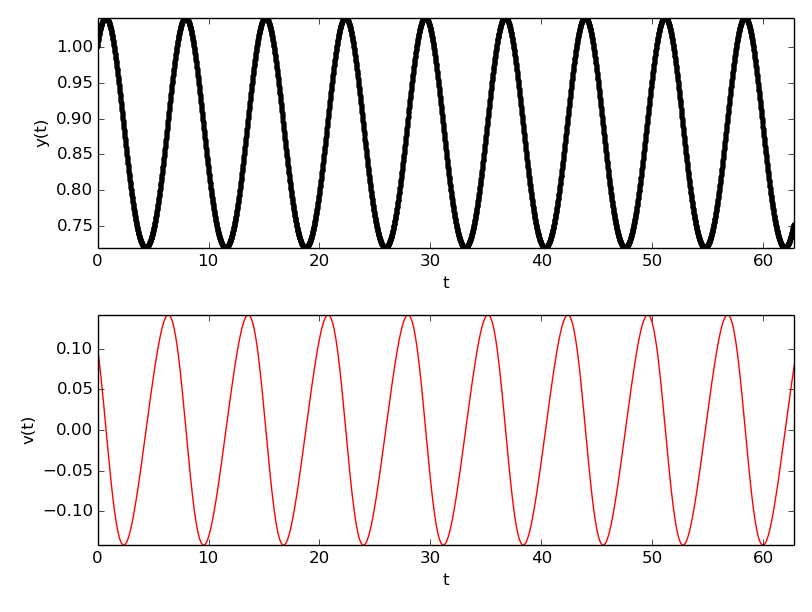
\includegraphics[width=0.75\textwidth]{images/gradB_ion_y}
     \caption{$y(t)$, $v_y(t)$ plot. We see again the expected sinusoidal motion of the ion along $y$, without any drift motion along $y$, as expected.}
\end{figure}

\begin{figure}[!ht]
  \centering
    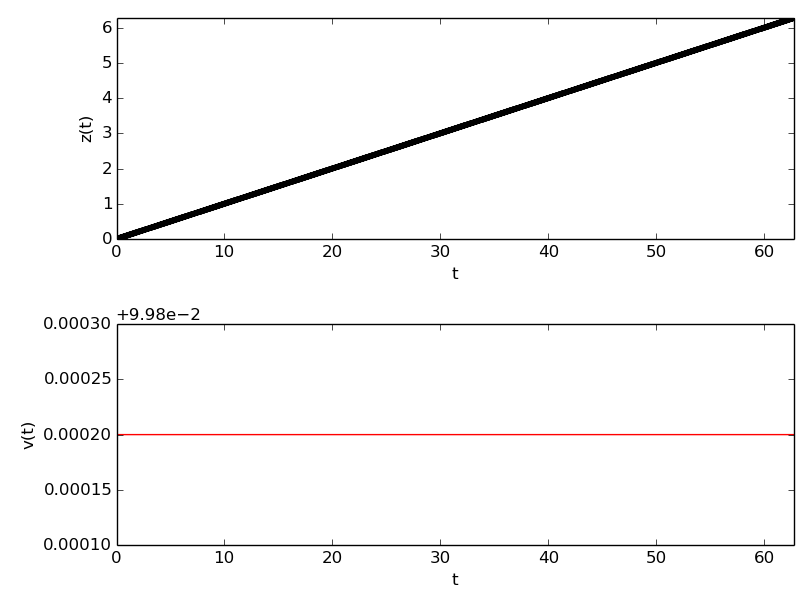
\includegraphics[width=0.75\textwidth]{images/gradB_ion_z}
     \caption{$z(t)$, $v_z(t)$ plot. The ion's motion along  is unaffected by the magnetic field, as expected. The ion moves along $z$ with its initial, constant velocity.}
\end{figure}

\begin{figure}[!ht]
  \centering
    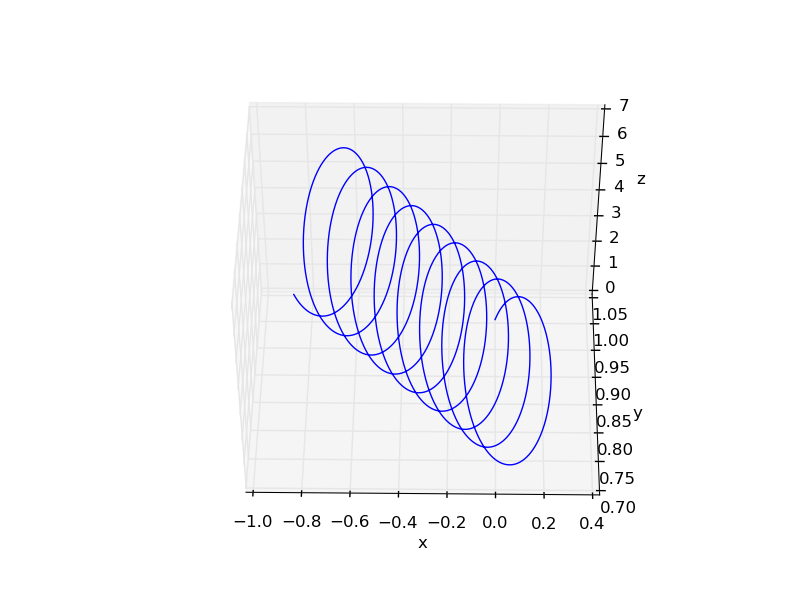
\includegraphics[width=0.75\textwidth]{images/gradB_ion_3d}
     \caption{The 3D plot of the ion's trajectory in a grad-B field. We see the expected helical motion plus the drift towards the negative $x$ axis.}
\end{figure}

\newpage

\section{Motion in a Magnetic Dipole Field}
The motion of a charged particle in a magnetic dipole field, which can be used to approximate the earth's magnetic field, is a very good example of charged particle motion. Inside a magnetic dipole field, a charged particle exhibits \emph{grad-B} and \emph{curvature B} drifts. A very good analysis and illustration of this kind of motion can be found in \cite{ozturk}.

The Earth's magnetic dipole field can be expressed in cartesian coordinates as:

\begin{equation}
\bm{B}_{dip} = - \frac{B_0 R_e^3}{r^5}\left[ 3xz \bm{\hat{x}} + 3yz \bm{\hat{y}} + (2z^2 -x^2 -y^2) \bm{\hat{z}} \right]
\end{equation}

where $B_0$ is the magnitude of the magnetic field at the equator and $R_e$ is the radius of the Earth. For simplicity, we will normalize both quantities to $1.0$ for the purposes of this example.
\newline

\newpage
We set up the magnetic field in \emph{src/fields.c} as follows, leaving the electric field set to zero:

\begin{lstlisting}
struct vector3D BField (struct vector3D r, double t)
{
  struct vector3D B;

  B.x = -(1.0/pow(sqrt(r.x*r.x+r.y*r.y+r.z*r.z),5))*3*r.x*r.z;
  B.y = -(1.0/pow(sqrt(r.x*r.x+r.y*r.y+r.z*r.z),5))*3*r.y*r.z;
  B.z = -(1.0/pow(sqrt(r.x*r.x+r.y*r.y+r.z*r.z),5))
  	     *(2*r.z*r.z-r.x*r.x-r.y*r.y);

  return B;
}
\end{lstlisting}

Afterwards, we set the initial conditions of the particle, to make sure that the particle is trapped in the magnetic field, as follows:

\begin{lstlisting}
r 0.075 0.0 0.0
v 2.0 2.0 12.0
\end{lstlisting}

Finally, we run the program:

\begin{lstlisting}
./cparticle i 0.8 0.000001 10
\end{lstlisting}

Below we can see the 3D plot of the particle's trajectory.

\begin{figure}[!ht]
  \centering
    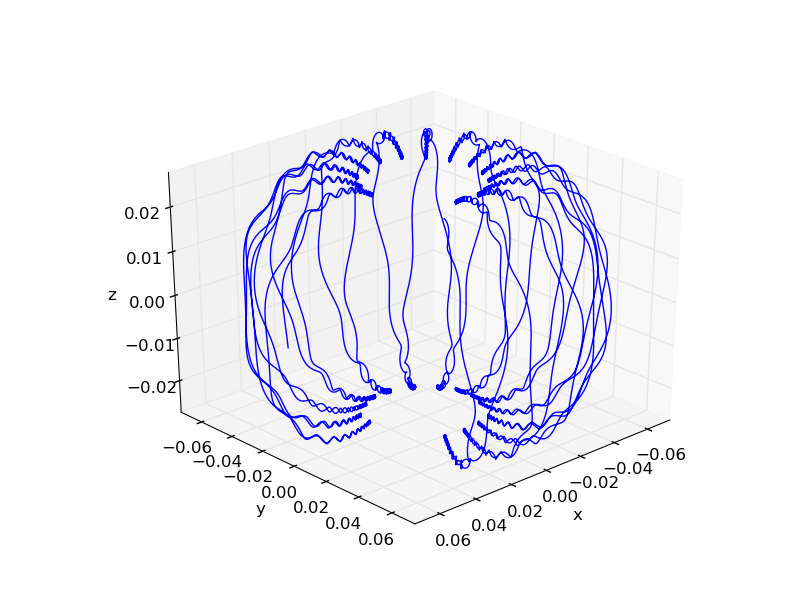
\includegraphics[width=0.75\textwidth]{images/earth_ion3d}
     \caption{The 3D plot of the ion's trajectory in a magnetic dipole field (similar to Earth's). We see the helical motion around the magnetic field lines, plus $\nabla B$ drift (north-south) along with \emph{curvature} drift (east-west).}
\end{figure}



\begin{thebibliography}{1}

  \bibitem{leveque} Randall J. LeVeque {\em Finite Difference Methods for Ordinary and Partial Differential Equations, }  2007.
  \bibitem{goldston} Robert J Goldston, Paul H Rutherford, {\em Introduction To Plasma Physics,}  1995.
  \bibitem{freidberg} Jeffrey Freidberg, {\em Plasma Physics and Fusion Energy,}  2007.
  \bibitem{bellan} Paul M. Bellan {\em Fundamentals of Plasma Physics,}  2006.
  \bibitem{ozturk} M. Kaan Ozturk, {\em Trajectories of charged particles trapped in Earth's magnetic field,}  2011.

  \end{thebibliography}

\end{document}